\section{Exrahieren von Gestenkandidaten}
\label{sec:gesture_extraction}
Die Lichtsensorenmatrix liefert einen kontinuierlichen Strom an Bildern. Als Gestenkandidat wird eine Folge von Bildern definiert, die
ein Ereignis einschließt. In diesem Fall wird das Ereignis durch die Veränderung im gleitenden Mittelwert der Helligkeit definiert. Sobald der gleitende Mittelwert unterschritten wird, wird ein Gestenkandidat
angefangen aufgenommen zu werden. Sobald die Lichtverhältnisse zu dem Wert zurückkehren, wird die Aufnahme beendet. Der gleitende Mittelwert wird immer angepasst, wenn kein Gestenkandidat aufgenommen wird, um
sich den verändernden Lichtverhältnissen anzupassen. Da leichte Veränderungen natürlich sind, muss eine Toleranzgrenze von 10\% unter- und überschritten werden, damit die Aufnahme gestartet, bzw. beendet wird.
Die Folge ist, dass der Anfang und das Ende nicht vollständig ist. Aus diesem Grund schlug Kubik zusätzlich vor am Anfang und Ende weitere Bilder anzufügen \cite{kubikThesis}.
\begin{figure}
    \usetikzlibrary{arrows,automata,positioning}
    \centering
    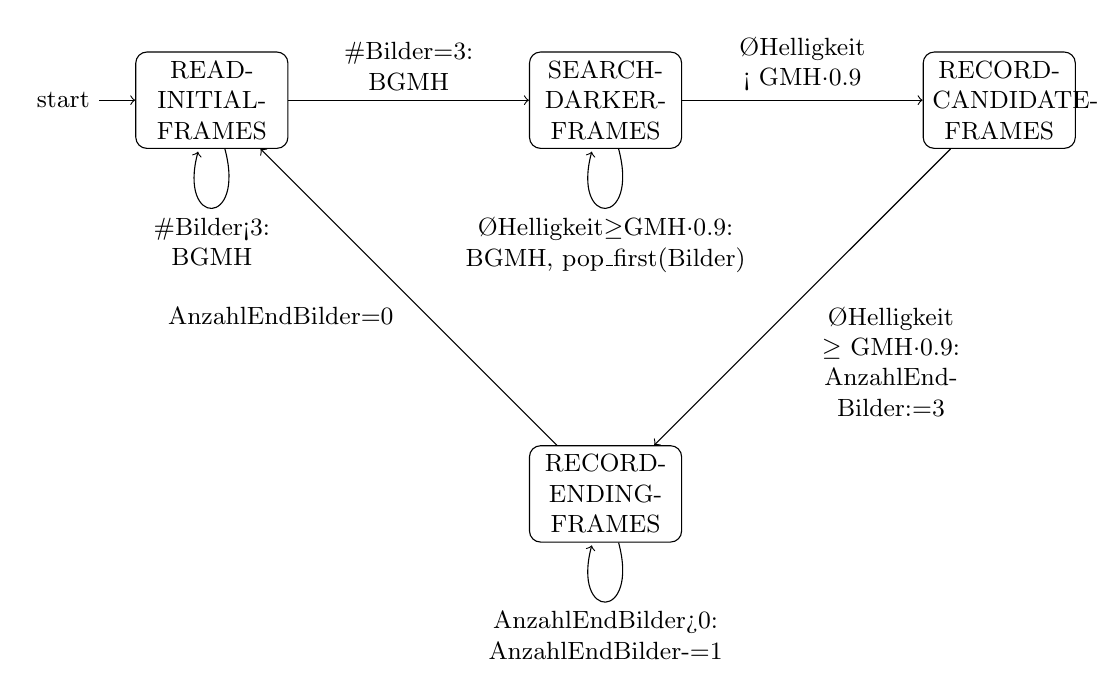
\begin{tikzpicture}[
        block/.style={
        draw,
        fill=white,
        text width=0.14*\columnwidth,
        anchor=west,
        minimum height=1cm,
        rounded corners
        },
        font=\small,
        on grid, auto,
        node distance=5cm
    ]
        \node [block,align=center,initial] (s0) {READ-INITIAL-FRAMES};
        \node [block,align=center] (s1) [right of=s0] {SEARCH-DARKER-FRAMES};
        \node [block,align=center] (s2) [right of=s1] {RECORD-CANDIDATE-FRAMES};
        \node [block,align=center] (s3) [below of=s1] {RECORD-ENDING-FRAMES};
        \path [->, text width=2cm, align=center] (s0) edge [loop below] node {\#Bilder<3: BGMH} (s0);
        \path [->, text width=2cm, align=center] (s0) edge node {\#Bilder=3: BGMH} (s1);
        \path [->, text width=4cm, align=center] (s1) edge [loop below] node {ØHelligkeit$\geq$GMH$\cdot 0.9$: BGMH, pop\_first(Bilder)} (s1);
        \path [->, text width=3cm, align=center] (s1) edge node {ØHelligkeit < GMH$\cdot 0.9$} (s2);
        \path [->, text width=2cm, align=center] (s2) edge node {ØHelligkeit $\geq$ GMH$\cdot 0.9$: AnzahlEndBilder:=3} (s3);
        \path [->, text width=3cm, align=center] (s3) edge [loop below] node {AnzahlEndBilder>0: AnzahlEndBilder-=1} (s3);
        \path [->, text width=3cm, align=center] (s3) edge node {AnzahlEndBilder=0} (s0);
    \end{tikzpicture}
    \caption{Die Implementierung von Dr. Marcus Venzke des Algorithmus von Kubik, um Gestenkandidaten zu erkennen. BGMH steht für die Aktion \glqq \textbf{B}erechnung \textbf{G}leitender \textbf{M}ittelwert der \textbf{H}elligkeit\grqq und GMH steht für die Variable \glqq \textbf{G}leitender \textbf{M}ittelwert der \textbf{H}elligkeit\grqq.}
    \label{fig:venzkeAlgoImpl}
\end{figure}
\newline
\newline
Abbildung \ref{fig:venzkeAlgoImpl} zeigt die konkrete Implementierung dieses Algorithmus mit einem Zustandsautomaten, der von Dr. Marcus Venzke entwickelt wurde. In jedem Zustand wird das aktuelle Bild dem Puffer angefügt.
Der Automat verbleibt im Zustand \texttt{READ-INITIAL-FRAMES} bis der Puffer drei Bilder enthält. Dabei wird stets der gleitende Mittelwert der Helligkeit angepasst. Anschließend geht der Automat in den Zustand
\texttt{SEARCH-DARKER-FRAMES} über, indem immer das erste Bild aus dem Puffer entfernt wird, da lediglich drei Bilder jeweils vor dem Aufnehmen und nach dem Aufnehmen des
Gestenkandidaten angefügt werden sollen. Außerdem wird weiterhin der gleitende Mittelwert angepasst. Sobald die Durchschnittshelligkeit 90\% des gleitenden Mittelwerts unterschreitet wird die Aufnahme begonnen.
Der Automat geht in den Zustand \texttt{RECORD-CANDIDATE-FRAMES} über. Dort verbleibt der Automat solange bis die Durchschnittshelligkeit 90\% des gleitenden Mittelwerts überschritten wird, woraufhin der Automat
in den Zustand \texttt{RECORD-ENDING-FRAMES} über geht. Dort werden die letzten drei Bilder dem Puffer angehängt. Sobald drei Bilder angehängt wurden, wird der Puffer dem Klassifizierer übergeben und anschließend
der Zustandsautomat zurückgesetzt. Daraufhin geht der Automat in den initialen Zustand wieder über.